\section{Beispielkapitel}
Dies ist ein Beispieltext.für

\subsection{Unterkapitel 1}\label{Unterkapitel1Link}
Beispiel für eine Fußnote\footnote{Fußnoten sind gut.}.

\begin{figure}[htbp]
	\centering
	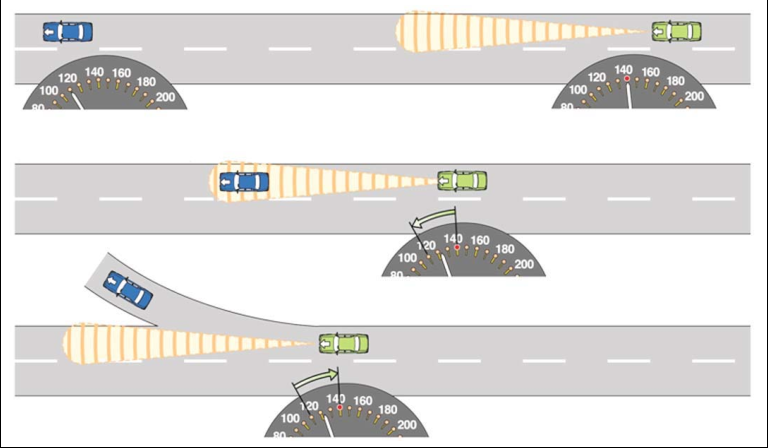
\includegraphics[width=1.0\textwidth]{pics/accBosch.pdf}
	\caption{Folgefahrt Beispielbild}
	\label{fig:accBosch}
\end{figure}

Wie in \ref{Unterkapitel1Link} gezeigt, ist es möglich, Kapitel zu verlinken. Abkürzungen wie das \ac{IfF} werden so dargestellt. Quellen übrigens so \citep{ams09}.

Abbildung ~\ref{fig:accBosch} soll ein Beispielhaftes Bild zeigen.


\subsubsection{Unterunterkapitel1} 

\textbf{\sffamily{Möglichkeit zur weiteren Unterteilung -- Teilkapitel}} Mehr als drei Unterteilungsebenen sollen vermieden werden!
\par
\begingroup
\leftskip=0.8cm
\noindent \textbf{\sffamily{Eingerücktes Teilkapitel}} Derartige Dinge wie eingerückte Teilkapitel gibt es auch. Falls Du sie brauchen solltest.
\par
\endgroup

\begin{table}[ht]
	\caption{Tabular Umgebung: Simpel formatierte Tabelle}
	\small
	\centering
	\begin{tabular}{ll}
		\toprule
		\multicolumn{2}{c}{Zwei miteinander verbundene Zellen}\\
		\midrule
		Punkt 1 & Adaptive Cruise Control\\
		Punkt 2 & Lane Keeping Assist\\			
		\toprule
		\multicolumn{2}{c}{Schon wieder zwei miteinander verbundene Zellen}\\
		\midrule
		Punkt 3 & Elektronisches Stabilitätsprogramm\\
		\toprule
	\end{tabular}
	\label{tab:Tabular1}
\end{table}

\begin{table}[h]
	\caption{Tabular Umgebung: Etwas komplexere Tabelle}
	\centering
	\begin{tabular}{|c|c|c|c|c|c|c|c|c|c|}
		\cline{2-10}
		\multicolumn{1}{c|}{} & \rotatebox{90}{Fahrzeug-CAN} & \rotatebox{90}{GPS-System} & \rotatebox{90}{ESP-Cluster} & \rotatebox{90}{Correvit} & \rotatebox{90}{Lichtschranke} & \rotatebox{90}{Radar} & \rotatebox{90}{Lidar} & \rotatebox{90}{Kreiselplattform} & \rotatebox{90}{Webcam, Leuchtdiode} \\
		\hline
		\multicolumn{10}{|c|}{}  \\
		\multicolumn{1}{|c}{\bfseries{Subjekt}} & \multicolumn{9}{c|}{}  \\
		\hline
		\hline	
		\multicolumn{1}{|c|}{Setzgeschwindigkeit}  &  &  &  &  &  &&  &  & x\\		
		\hline	
		\multicolumn{10}{|c|}{}  \\
		\multicolumn{1}{|c}{\bfseries{relative Größen}} & \multicolumn{9}{c|}{}  \\
		\hline
		\multicolumn{1}{|c|}{Triggersignal}  &  & x &   &  & x &   &  & & x \\		
		\hline	
		\multicolumn{10}{|c|}{}  \\
		\multicolumn{1}{|c}{\bfseries{Objekt}} & \multicolumn{9}{c|}{}  \\
		\hline
		\multicolumn{1}{|c|}{Längsgeschwindigkeit} & x  & x &  & x &   &  &&   &    \\	
		\hline
	\end{tabular}
	\label{tab:sensorik}
\end{table}

Nachfolgend das Beispiel für eine Aufzählung mit Itemize.
\begin{itemize}
	\item Reaktionszeit $\mathrm{\Delta t_{react}}$
	\item Im oberen Punkt sieht man auch schön die Einbindung von Formeln in den Text.
\end{itemize}

$v_{Obj.}$ = 120\,km/h \\
Einheiten sollten nicht kursiv dargestellt werden und werden vom Zahlenwert durch ein schmales Leerzeichen (Backslash und Komma) getrennt.

Es gibt eine Vielzahl von Gleichungsumgebungen. Equation ist eine davon. Die Gleichung ergibt natürlich keinen tieferen Sinn:
\begin{equation}
	x_{obj} = \frac{s^{2} \cdot a \cdot \sqrt{b}}{234 \cdot h_{ego}}
\end{equation}

